%
% Der Satz von Gauss
%
\section{Der verallgemeinerte Satz von Gauss
\label{buch:gauss:section:satzvongauss}}
\kopfrechts{Der verallgemeinerte Satz von Gauss}
Der Fall $n=3$ ist nicht speziell.
Die Theorie von Abschnitt~\ref{buch:gauss:section:dimension3}
kann auf beliebige $n$-dimensionale Mannigfaltigkeiten mit Rand
verallgemeinert werden.
In diesem Abschnitt ist daher $V$ eine $n$-dimensionale Mannigfaltigkeit.

% 
% n-Vektoren und n-Formen
%
\subsection{$n$-Vektoren und $n$-Formen}
Das Levi-Cività-Symbol kann verwendet werden, um den eindimensionalen
Raum der $n$-Vektoren mit dem Basisvektor
\[
\vec{e}_1\wedge\dots\wedge \vec{e}_n
=
\sum_{i_1,\dots,i_n=1}^n
\varepsilon_{i_1\dots i_n}
\,
\vec{e}_{i_1}\otimes\dots\otimes\vec{e}_{i_n}
\]
aufzuspannen.

Dual dazu ist eine $n$-Form das Produkt
\[
\omega
=
f(x)
\,
dx^1\wedge\dots\wedge dx^n.
\]
Wie im Fall $n=3$ kann man zeigen, dass das Transformationsgesetz
für eine solche $n$-Form die Multiplikation mit der Determinante
der $n\times n$-Matrix $Dy$ ist.
Dies ist die Funktionaldeterminanten einer $n$-dimensionalen
Koordinatentransformation.

%
% n-1-Vektoren und n-1-Formen
%
\subsection{$n-1$-Vektoren und $n-1$-Formen}
$n-1$-Vektoren sind Linearkombinationen
\[
\sum_{1\le i_1<\dots<i_{n-1}\le n}
a_{i_1\dots i_{n-1}}
\vec{e}_{i_1}\wedge\dots\wedge \vec{e}_{i_{n-1}}
\]
von $\wedge$-Produkt von jeweils $n-1$ Vektoren aus den Basisvektoren
$\vec{e}_1,\dots\vec{e}_n$.
Ein Basis-$n-1$-Vektor ist ein $\wedge$-Produkt von $n-1$ von den $n$
Basisvektoren.
Er stellt ein $n-1$-dimensionales Parallelepiped dar, welches senkrecht
auf der Richtung des fehlenden Vektors steht.

Im Fall $n=3$ messen 2-Formen die Projektion eines Parallelogramms
oder 2-Vektors auf die Ebene, die zu dieser 2-Form gehört.
Die Basis-2-Formen entstehen als Wedge-Produkt
\[
dx^1\wedge\dots\wedge \widehat{dx^i}\wedge\dots\wedge dx^n
\]
von $n-1$ Basis-1-Formen, wobei genau eine der 1-Formen fehlt,
nämlich die durch den Hut gekennzeichnete 1-Form $dx^i$.
Die fehlende 1-Form gehört zur Richtung senkrecht auf das
$n-1$-dimensionale Parallelepiped, das von den anderen Vektoren
aufgespannt wird.

%
% Die äussere Ableitung
%
\subsection{Die äussere Ableitung}
Für die Formulierung des Satzes von Gauss wird ausserdem die
äussere Ableitung eine $n-1$-Form benötigt.
Da der Operator der äusseren Ableitung linear ist, muss er nur
auf Basis-$n-1$-Formen definiert werden.
Wir betrachten daher die $n-1$-Form
\[
\alpha
=
a_i(x)\, dx^1\wedge\dots\wedge \widehat{dx^i}\wedge\dots\wedge dx^n.
\]
Die äussere Ableitung leitete nach der Variablen $x^i$ ab und fügt
die 1-Form $dx^i$ zum Wedge-Produkt hinzu.
Wie im Fall $n=3$ muss das Vorzeichen jeweils so angepasst werden,
dass die Orientierung der $n-1$-Form mit der Orientierung
$dx^1\wedge\dots\wedge dx^n$ kompatibel ist.
Daher muss
\begin{equation}
d\alpha
=
(-1)^{i-1}
\frac{\partial a_i(x)}{\partial x^i}
\,
dx^1\wedge\dots\wedge dx^n
\label{buch:gauss:nd:eqn:d}
\end{equation}
gesetzt werden.
Man kann dies auch wie folgt definieren.

\begin{definition}
Die {\em äussere Ableitung} der $n-1$-Form
\[
\alpha = a(x)\, dx^{i_1}\wedge\dots\wedge dx^{i_{n-1}}
\]
ist
\begin{equation}
d\alpha
=
\frac{\partial a}{\partial x^i}(x)
\,dx^i
\wedge dx^{i_1}\wedge\dots\wedge dx^{i_{n-1}}.
\label{buch:gauss:nd:eqn:dabl}
\end{equation}
\end{definition}

Da der Raum der $n$-Formen eindimensional ist, kann 
das Wedge-Produkt in \eqref{buch:gauss:nd:eqn:dabl}
immer so umgestellt werden, dass die $n$-Form
$dx^1\wedge\dots\wedge dx^n$ entsteht.
Im Falle der $n-1$-Form
\[
dx^1\wedge\dots\wedge\widehat{dx^i}\wedge\dots\wedge dx^n
\]
bedeutet dies, dass die 1-Form $dx^i$ in
\[
dx^i
\wedge
dx^1\wedge\dots\wedge\widehat{dx^i}\wedge\dots\wedge dx^n
\]
mit $i-1$ Vertauschungen an den ``richtigen'' Platz gebracht
werden kann.
Dies bringt ein Vorzeichen $(-1)^{i-1}$, welches auch in
\eqref{buch:gauss:nd:eqn:d}
wiedergefunden werden kann.

%
% Der Satz von Gauss
%
\subsection{Der Satz von Gauss
\label{buch:gauss:gauss:subsection:satzvongauss}}
\kopfrechts{Der Satz von Gauss}
Der Satz von Gauss kann jetzt für beliebige Dimension $n$ formuliert
werden.
Auf einer $n$-dimensionalen Mannigfaltigkeit ist die Integration
einer $n$-Form definiert.
Der Rand einer $n$-dimensionalen Mannigfaltigkeit ist $n-1$-dimensional,
auf dem Rand ist daher die Integration einer $n-1$-Form definiert.
Eine $n-1$-Form $\omega$ auf der Mannigfaltigkeit hat als äussere 
Ableitung eine $n$-Form $d\omega$.
Der Satz von Gauss verbindet das $n$-Form-Integral von $d\alpha$
über die ganze Mannigfaltigkeit mit dem $n-1$-Form-Integral von $\alpha$
über den Rand der Mannigfaltigkeit.

\begin{satz}[Gauss]
Sei $M$ eine $n$-dimensionale Mannigfaltigkeit mit Rand $\partial M$
und $\omega$ eine $n-1$-Form auf $M$.
Dann gilt
\[
\int_M d\omega
=
\int_{\partial M} \omega.
\]
\end{satz}

%
% fig-kuh.tex
%
% (c) 2025 Prof Dr Andreas Müller
%
\begin{figure}
\centering
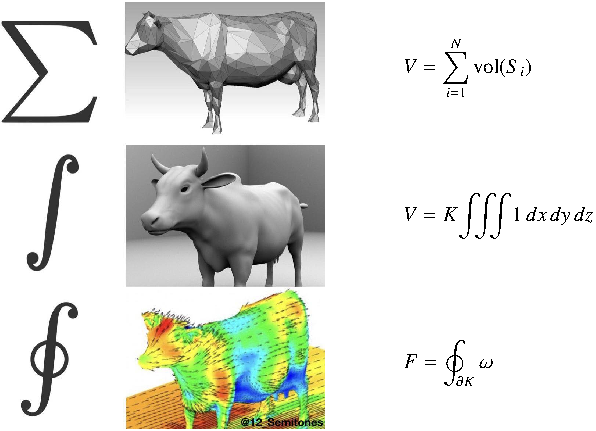
\includegraphics{chapters/050-gauss/images/kuh.pdf}
\caption{Internet-Meme, welches den Unterschied zwischen diskreter
Volumenberechnung, Volumenintegral und Flussintegral über die
Oberfläche eines Körpers illustriert.
\label{buch:gauss:fig:kuh}}
\end{figure}
%
Das Internet-Meme vom Abbildung~\ref{buch:gauss:fig:kuh} versucht,
die Idee des Integrals über den Rand einer Mannigfaltigkeit
mit Rand humoristisch zu interpretieren.
Tatsächlich ist ein solches Integral nicht nur für den Satz von Gauss
von Nutzen.
In der Elastizitätstheorie geht man davon aus, dass auf einem Element
der Oberfläche, also auf einem infinitesimalen 2-Vektor, sowohl Druckkräfte
orthogonal auf das Parallelepiped wirken, als auch Scherkräfte parallel 
zur Ebene des Parallelepipeds.
Das Integral dieser Kräfte ergibt die resultierende Kraft auf den Körper.
Die Kräfte haben auch Drehmomente zur Folge.
Falls sich der Körper nicht in Drehbewegung versetzen kann, muss
das Integral dieser Drehmomente über die ganze Oberfläche
Null ergeben.

